% Created by tikzDevice version 0.8.1 on 2015-11-17 12:57:39
% !TEX encoding = UTF-8 Unicode
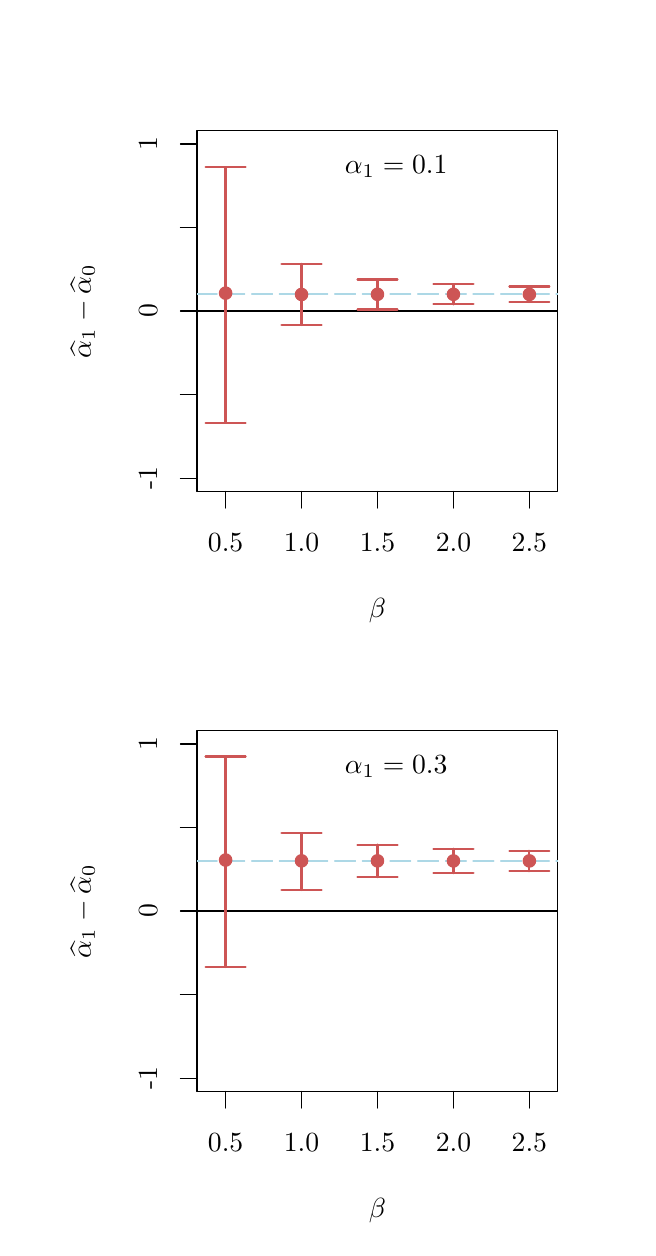
\begin{tikzpicture}[x=1pt,y=1pt]
\definecolor{fillColor}{RGB}{255,255,255}
\path[use as bounding box,fill=fillColor,fill opacity=0.00] (0,0) rectangle (216.81,433.62);
\begin{scope}
\path[clip] (  0.00,  0.00) rectangle (216.81,433.62);
\definecolor{drawColor}{RGB}{0,0,0}

\path[draw=drawColor,line width= 0.4pt,line join=round,line cap=round] ( 71.52,266.01) -- (181.29,266.01);

\path[draw=drawColor,line width= 0.4pt,line join=round,line cap=round] ( 71.52,266.01) -- ( 71.52,260.01);

\path[draw=drawColor,line width= 0.4pt,line join=round,line cap=round] ( 98.96,266.01) -- ( 98.96,260.01);

\path[draw=drawColor,line width= 0.4pt,line join=round,line cap=round] (126.40,266.01) -- (126.40,260.01);

\path[draw=drawColor,line width= 0.4pt,line join=round,line cap=round] (153.85,266.01) -- (153.85,260.01);

\path[draw=drawColor,line width= 0.4pt,line join=round,line cap=round] (181.29,266.01) -- (181.29,260.01);

\node[text=drawColor,anchor=base,inner sep=0pt, outer sep=0pt, scale=  1.00] at ( 71.52,244.41) {0.5};

\node[text=drawColor,anchor=base,inner sep=0pt, outer sep=0pt, scale=  1.00] at ( 98.96,244.41) {1.0};

\node[text=drawColor,anchor=base,inner sep=0pt, outer sep=0pt, scale=  1.00] at (126.40,244.41) {1.5};

\node[text=drawColor,anchor=base,inner sep=0pt, outer sep=0pt, scale=  1.00] at (153.85,244.41) {2.0};

\node[text=drawColor,anchor=base,inner sep=0pt, outer sep=0pt, scale=  1.00] at (181.29,244.41) {2.5};

\path[draw=drawColor,line width= 0.4pt,line join=round,line cap=round] ( 61.20,266.01) --
	(191.61,266.01) --
	(191.61,396.42) --
	( 61.20,396.42) --
	( 61.20,266.01);
\end{scope}
\begin{scope}
\path[clip] (  0.00,216.81) rectangle (216.81,433.62);
\definecolor{drawColor}{RGB}{0,0,0}

\node[text=drawColor,anchor=base,inner sep=0pt, outer sep=0pt, scale=  1.00] at (126.41,220.41) {$\beta$};

\node[text=drawColor,rotate= 90.00,anchor=base,inner sep=0pt, outer sep=0pt, scale=  1.00] at ( 22.80,331.22) {$\widehat{\alpha}_1 - \widehat{\alpha}_0$};
\end{scope}
\begin{scope}
\path[clip] (  0.00,  0.00) rectangle (216.81,433.62);
\definecolor{drawColor}{RGB}{0,0,0}

\path[draw=drawColor,line width= 0.4pt,line join=round,line cap=round] ( 61.20,270.84) -- ( 61.20,391.59);

\path[draw=drawColor,line width= 0.4pt,line join=round,line cap=round] ( 61.20,270.84) -- ( 55.20,270.84);

\path[draw=drawColor,line width= 0.4pt,line join=round,line cap=round] ( 61.20,301.03) -- ( 55.20,301.03);

\path[draw=drawColor,line width= 0.4pt,line join=round,line cap=round] ( 61.20,331.22) -- ( 55.20,331.22);

\path[draw=drawColor,line width= 0.4pt,line join=round,line cap=round] ( 61.20,361.40) -- ( 55.20,361.40);

\path[draw=drawColor,line width= 0.4pt,line join=round,line cap=round] ( 61.20,391.59) -- ( 55.20,391.59);

\node[text=drawColor,rotate= 90.00,anchor=base,inner sep=0pt, outer sep=0pt, scale=  1.00] at ( 46.80,270.84) {-1};

\node[text=drawColor,rotate= 90.00,anchor=base,inner sep=0pt, outer sep=0pt, scale=  1.00] at ( 46.80,331.22) {0};

\node[text=drawColor,rotate= 90.00,anchor=base,inner sep=0pt, outer sep=0pt, scale=  1.00] at ( 46.80,391.59) {1};
\end{scope}
\begin{scope}
\path[clip] ( 61.20,266.01) rectangle (191.61,396.42);
\definecolor{drawColor}{RGB}{0,0,0}

\node[text=drawColor,anchor=base west,inner sep=0pt, outer sep=0pt, scale=  1.00] at (114.66,380.98) {$\alpha_1=0.1$};
\definecolor{drawColor}{RGB}{173,216,230}

\path[draw=drawColor,line width= 0.8pt,dash pattern=on 7pt off 3pt ,line join=round,line cap=round] ( 61.20,337.25) -- (191.61,337.25);

\path[draw=drawColor,line width= 0.8pt,dash pattern=on 7pt off 3pt ,line join=round,line cap=round] ( 61.20,337.25) -- (191.61,337.25);

\path[draw=drawColor,line width= 0.8pt,dash pattern=on 7pt off 3pt ,line join=round,line cap=round] ( 61.20,337.25) -- (191.61,337.25);

\path[draw=drawColor,line width= 0.8pt,dash pattern=on 7pt off 3pt ,line join=round,line cap=round] ( 61.20,337.25) -- (191.61,337.25);

\path[draw=drawColor,line width= 0.8pt,dash pattern=on 7pt off 3pt ,line join=round,line cap=round] ( 61.20,337.25) -- (191.61,337.25);
\definecolor{drawColor}{RGB}{0,0,0}

\path[draw=drawColor,line width= 0.4pt,line join=round,line cap=round] ( 61.20,331.22) -- (191.61,331.22);
\definecolor{drawColor}{RGB}{205,85,85}

\path[draw=drawColor,line width= 0.8pt,line join=round,line cap=round] ( 71.52,290.82) -- ( 71.52,383.23);

\path[draw=drawColor,line width= 0.8pt,line join=round,line cap=round] ( 64.29,290.82) --
	( 71.52,290.82) --
	( 78.75,290.82);

\path[draw=drawColor,line width= 0.8pt,line join=round,line cap=round] ( 78.75,383.23) --
	( 71.52,383.23) --
	( 64.29,383.23);

\path[draw=drawColor,line width= 0.8pt,line join=round,line cap=round] ( 98.96,326.17) -- ( 98.96,348.25);

\path[draw=drawColor,line width= 0.8pt,line join=round,line cap=round] ( 91.73,326.17) --
	( 98.96,326.17) --
	(106.19,326.17);

\path[draw=drawColor,line width= 0.8pt,line join=round,line cap=round] (106.19,348.25) --
	( 98.96,348.25) --
	( 91.73,348.25);

\path[draw=drawColor,line width= 0.8pt,line join=round,line cap=round] (126.40,331.79) -- (126.40,342.65);

\path[draw=drawColor,line width= 0.8pt,line join=round,line cap=round] (119.18,331.79) --
	(126.40,331.79) --
	(133.63,331.79);

\path[draw=drawColor,line width= 0.8pt,line join=round,line cap=round] (133.63,342.65) --
	(126.40,342.65) --
	(119.18,342.65);

\path[draw=drawColor,line width= 0.8pt,line join=round,line cap=round] (153.85,333.63) -- (153.85,340.92);

\path[draw=drawColor,line width= 0.8pt,line join=round,line cap=round] (146.62,333.63) --
	(153.85,333.63) --
	(161.08,333.63);

\path[draw=drawColor,line width= 0.8pt,line join=round,line cap=round] (161.08,340.92) --
	(153.85,340.92) --
	(146.62,340.92);

\path[draw=drawColor,line width= 0.8pt,line join=round,line cap=round] (181.29,334.45) -- (181.29,340.07);

\path[draw=drawColor,line width= 0.8pt,line join=round,line cap=round] (174.06,334.45) --
	(181.29,334.45) --
	(188.52,334.45);

\path[draw=drawColor,line width= 0.8pt,line join=round,line cap=round] (188.52,340.07) --
	(181.29,340.07) --
	(174.06,340.07);
\definecolor{fillColor}{RGB}{205,85,85}

\path[draw=drawColor,line width= 0.4pt,line join=round,line cap=round,fill=fillColor] ( 71.52,337.69) circle (  2.25);

\path[draw=drawColor,line width= 0.4pt,line join=round,line cap=round,fill=fillColor] ( 98.96,337.21) circle (  2.25);

\path[draw=drawColor,line width= 0.4pt,line join=round,line cap=round,fill=fillColor] (126.40,337.26) circle (  2.25);

\path[draw=drawColor,line width= 0.4pt,line join=round,line cap=round,fill=fillColor] (153.85,337.26) circle (  2.25);

\path[draw=drawColor,line width= 0.4pt,line join=round,line cap=round,fill=fillColor] (181.29,337.23) circle (  2.25);
\end{scope}
\begin{scope}
\path[clip] (  0.00,  0.00) rectangle (216.81,433.62);
\definecolor{drawColor}{RGB}{0,0,0}

\path[draw=drawColor,line width= 0.4pt,line join=round,line cap=round] ( 71.52, 49.20) -- (181.29, 49.20);

\path[draw=drawColor,line width= 0.4pt,line join=round,line cap=round] ( 71.52, 49.20) -- ( 71.52, 43.20);

\path[draw=drawColor,line width= 0.4pt,line join=round,line cap=round] ( 98.96, 49.20) -- ( 98.96, 43.20);

\path[draw=drawColor,line width= 0.4pt,line join=round,line cap=round] (126.40, 49.20) -- (126.40, 43.20);

\path[draw=drawColor,line width= 0.4pt,line join=round,line cap=round] (153.85, 49.20) -- (153.85, 43.20);

\path[draw=drawColor,line width= 0.4pt,line join=round,line cap=round] (181.29, 49.20) -- (181.29, 43.20);

\node[text=drawColor,anchor=base,inner sep=0pt, outer sep=0pt, scale=  1.00] at ( 71.52, 27.60) {0.5};

\node[text=drawColor,anchor=base,inner sep=0pt, outer sep=0pt, scale=  1.00] at ( 98.96, 27.60) {1.0};

\node[text=drawColor,anchor=base,inner sep=0pt, outer sep=0pt, scale=  1.00] at (126.40, 27.60) {1.5};

\node[text=drawColor,anchor=base,inner sep=0pt, outer sep=0pt, scale=  1.00] at (153.85, 27.60) {2.0};

\node[text=drawColor,anchor=base,inner sep=0pt, outer sep=0pt, scale=  1.00] at (181.29, 27.60) {2.5};

\path[draw=drawColor,line width= 0.4pt,line join=round,line cap=round] ( 61.20, 49.20) --
	(191.61, 49.20) --
	(191.61,179.61) --
	( 61.20,179.61) --
	( 61.20, 49.20);
\end{scope}
\begin{scope}
\path[clip] (  0.00,  0.00) rectangle (216.81,216.81);
\definecolor{drawColor}{RGB}{0,0,0}

\node[text=drawColor,anchor=base,inner sep=0pt, outer sep=0pt, scale=  1.00] at (126.41,  3.60) {$\beta$};

\node[text=drawColor,rotate= 90.00,anchor=base,inner sep=0pt, outer sep=0pt, scale=  1.00] at ( 22.80,114.41) {$\widehat{\alpha}_1 - \widehat{\alpha}_0$};
\end{scope}
\begin{scope}
\path[clip] (  0.00,  0.00) rectangle (216.81,433.62);
\definecolor{drawColor}{RGB}{0,0,0}

\path[draw=drawColor,line width= 0.4pt,line join=round,line cap=round] ( 61.20, 54.03) -- ( 61.20,174.78);

\path[draw=drawColor,line width= 0.4pt,line join=round,line cap=round] ( 61.20, 54.03) -- ( 55.20, 54.03);

\path[draw=drawColor,line width= 0.4pt,line join=round,line cap=round] ( 61.20, 84.22) -- ( 55.20, 84.22);

\path[draw=drawColor,line width= 0.4pt,line join=round,line cap=round] ( 61.20,114.41) -- ( 55.20,114.41);

\path[draw=drawColor,line width= 0.4pt,line join=round,line cap=round] ( 61.20,144.59) -- ( 55.20,144.59);

\path[draw=drawColor,line width= 0.4pt,line join=round,line cap=round] ( 61.20,174.78) -- ( 55.20,174.78);

\node[text=drawColor,rotate= 90.00,anchor=base,inner sep=0pt, outer sep=0pt, scale=  1.00] at ( 46.80, 54.03) {-1};

\node[text=drawColor,rotate= 90.00,anchor=base,inner sep=0pt, outer sep=0pt, scale=  1.00] at ( 46.80,114.41) {0};

\node[text=drawColor,rotate= 90.00,anchor=base,inner sep=0pt, outer sep=0pt, scale=  1.00] at ( 46.80,174.78) {1};
\end{scope}
\begin{scope}
\path[clip] ( 61.20, 49.20) rectangle (191.61,179.61);
\definecolor{drawColor}{RGB}{0,0,0}

\node[text=drawColor,anchor=base west,inner sep=0pt, outer sep=0pt, scale=  1.00] at (114.66,164.17) {$\alpha_1=0.3$};
\definecolor{drawColor}{RGB}{173,216,230}

\path[draw=drawColor,line width= 0.8pt,dash pattern=on 7pt off 3pt ,line join=round,line cap=round] ( 61.20,132.52) -- (191.61,132.52);

\path[draw=drawColor,line width= 0.8pt,dash pattern=on 7pt off 3pt ,line join=round,line cap=round] ( 61.20,132.52) -- (191.61,132.52);

\path[draw=drawColor,line width= 0.8pt,dash pattern=on 7pt off 3pt ,line join=round,line cap=round] ( 61.20,132.52) -- (191.61,132.52);

\path[draw=drawColor,line width= 0.8pt,dash pattern=on 7pt off 3pt ,line join=round,line cap=round] ( 61.20,132.52) -- (191.61,132.52);

\path[draw=drawColor,line width= 0.8pt,dash pattern=on 7pt off 3pt ,line join=round,line cap=round] ( 61.20,132.52) -- (191.61,132.52);
\definecolor{drawColor}{RGB}{0,0,0}

\path[draw=drawColor,line width= 0.4pt,line join=round,line cap=round] ( 61.20,114.41) -- (191.61,114.41);
\definecolor{drawColor}{RGB}{205,85,85}

\path[draw=drawColor,line width= 0.8pt,line join=round,line cap=round] ( 71.52, 94.21) -- ( 71.52,170.29);

\path[draw=drawColor,line width= 0.8pt,line join=round,line cap=round] ( 64.29, 94.21) --
	( 71.52, 94.21) --
	( 78.75, 94.21);

\path[draw=drawColor,line width= 0.8pt,line join=round,line cap=round] ( 78.75,170.29) --
	( 71.52,170.29) --
	( 64.29,170.29);

\path[draw=drawColor,line width= 0.8pt,line join=round,line cap=round] ( 98.96,122.02) -- ( 98.96,142.54);

\path[draw=drawColor,line width= 0.8pt,line join=round,line cap=round] ( 91.73,122.02) --
	( 98.96,122.02) --
	(106.19,122.02);

\path[draw=drawColor,line width= 0.8pt,line join=round,line cap=round] (106.19,142.54) --
	( 98.96,142.54) --
	( 91.73,142.54);

\path[draw=drawColor,line width= 0.8pt,line join=round,line cap=round] (126.40,126.68) -- (126.40,138.40);

\path[draw=drawColor,line width= 0.8pt,line join=round,line cap=round] (119.18,126.68) --
	(126.40,126.68) --
	(133.63,126.68);

\path[draw=drawColor,line width= 0.8pt,line join=round,line cap=round] (133.63,138.40) --
	(126.40,138.40) --
	(119.18,138.40);

\path[draw=drawColor,line width= 0.8pt,line join=round,line cap=round] (153.85,128.12) -- (153.85,136.92);

\path[draw=drawColor,line width= 0.8pt,line join=round,line cap=round] (146.62,128.12) --
	(153.85,128.12) --
	(161.08,128.12);

\path[draw=drawColor,line width= 0.8pt,line join=round,line cap=round] (161.08,136.92) --
	(153.85,136.92) --
	(146.62,136.92);

\path[draw=drawColor,line width= 0.8pt,line join=round,line cap=round] (181.29,128.74) -- (181.29,136.25);

\path[draw=drawColor,line width= 0.8pt,line join=round,line cap=round] (174.06,128.74) --
	(181.29,128.74) --
	(188.52,128.74);

\path[draw=drawColor,line width= 0.8pt,line join=round,line cap=round] (188.52,136.25) --
	(181.29,136.25) --
	(174.06,136.25);
\definecolor{fillColor}{RGB}{205,85,85}

\path[draw=drawColor,line width= 0.4pt,line join=round,line cap=round,fill=fillColor] ( 71.52,132.84) circle (  2.25);

\path[draw=drawColor,line width= 0.4pt,line join=round,line cap=round,fill=fillColor] ( 98.96,132.55) circle (  2.25);

\path[draw=drawColor,line width= 0.4pt,line join=round,line cap=round,fill=fillColor] (126.40,132.55) circle (  2.25);

\path[draw=drawColor,line width= 0.4pt,line join=round,line cap=round,fill=fillColor] (153.85,132.52) circle (  2.25);

\path[draw=drawColor,line width= 0.4pt,line join=round,line cap=round,fill=fillColor] (181.29,132.53) circle (  2.25);
\end{scope}
\end{tikzpicture}
